%%%%%%%%%%%%%%%%%%%%%%%%%%% asme2ej.tex %%%%%%%%%%%%%%%%%%%%%%%%%%%%%%%
% Template for producing ASME-format journal articles using LaTeX    %
% Written by   Harry H. Cheng, Professor and Director                %
%              Integration Engineering Laboratory                    %
%              Department of Mechanical and Aeronautical Engineering %
%              University of California                              %
%              Davis, CA 95616                                       %
%              Tel: (530) 752-5020 (office)                          %
%                   (530) 752-1028 (lab)                             %
%              Fax: (530) 752-4158                                   %
%              Email: hhcheng@ucdavis.edu                            %
%              WWW:   http://iel.ucdavis.edu/people/cheng.html       %
%              May 7, 1994                                           %
% Modified: February 16, 2001 by Harry H. Cheng                      %
% Modified: January  01, 2003 by Geoffrey R. Shiflett                %
% Butchered: October 15, 2014 by John Karasinski                %
% Use at your own risk, send complaints to /dev/null                 %
%%%%%%%%%%%%%%%%%%%%%%%%%%%%%%%%%%%%%%%%%%%%%%%%%%%%%%%%%%%%%%%%%%%%%%

%%% use twocolumn and 10pt options with the asme2ej format
\documentclass[twocolumn,10pt]{asme2ej}

\usepackage{epsfig} %% for loading postscript figures
\usepackage{listings}
\usepackage{amsmath}
\usepackage{graphicx}
\usepackage{grffile}
\usepackage{pdfpages}
\usepackage{algpseudocode}

%% The class has several options
%  onecolumn/twocolumn - format for one or two columns per page
%  10pt/11pt/12pt - use 10, 11, or 12 point font
%  oneside/twoside - format for oneside/twosided printing
%  final/draft - format for final/draft copy
%  cleanfoot - take out copyright info in footer leave page number
%  cleanhead - take out the conference banner on the title page
%  titlepage/notitlepage - put in titlepage or leave out titlepage
%
%% The default is oneside, onecolumn, 10pt, final

\title{Case Study \# 1: 1D Transient Heat Diffusion}

%%% first author
\author{John Karasinski
    \affiliation{
	Graduate Student Researcher\\
	Center for Human/Robotics/Vehicle Integration and Performance\\
	Department of Mechanical and Aerospace Engineering\\
	University of California\\
	Davis, California 95616\\
    Email: karasinski@ucdavis.edu
    }
}

\begin{document}
\maketitle

%%%%%%%%%%%%%%%%%%%%%%%%%%%%%%%%%%%%%%%%%%%%%%%%%%%%%%%%%%%%%%%%%%%%%%
\section{Problem Description}

The problem of 1D unsteady heat diffusion in a slab of unit length with a zero initial temperature and both ends maintained at a unit temperature can be described by:
\begin{equation}
\frac{\partial T}{\partial t} = \frac{\partial^2T}{\partial x^2} \mbox{ subject to } \left\{ \begin{array}{lll}
        \mbox{$T(x, 0^-)= 0 $} & \mbox{for } &0 \leq x \leq 1 \\
        \mbox{$T(0, t) = T(1, t) = 1$} & \mbox{for } &t > 0 \end{array} \right.
\label{eq_DEF}
\end{equation}
\noindent and has the well known analytical solution:
\begin{equation}
\begin{split}
T^*(x,t) = 1 - \sum\limits_{k=1}^\infty \frac{4}{(2k-1)\pi} & \sin[(2k-1)\pi x] \star \\
		    &  \exp[-(2k-1)^2\pi^2t].
\end{split}
\end{equation}

In addition to the analytical solution, several numerical methods can be employed to solve the diffusion equation. Two of these methods, both an explicit and an implicit scheme, are derived in the following section. A Python script was then used to obtain results for a 21 point mesh (N=21) along the slab, and the Root Mean Square error,
\begin{equation}
\mbox{RMS} = \frac{1}{N^\frac{1}{2}}\sqrt{\sum\limits_{i=1}^N[T_i^n - T^*(x_i, t_n)]^2}
\end{equation}
was obtained for $s(=\Delta t/ \Delta x^2)$ = 1/6, 0.25, 0.5, and 0.75, at $t$ = 0.03, 0.06, and 0.09 using both the explicit and the implicit methods.

%%%%%%%%%%%%%%%%%%%%%%%%%%%%%%%%%%%%%%%%%%%%%%%%%%%%%%%%%%%%%%%%%%%%%%
\section{Solution Algorithms}

The Taylor-series (TS) method can be used on this equation to derive a finite difference approximation to the PDE. Applying the definition of the derivative,
\begin{equation}
f'(x) \approx \frac{f(x + \epsilon) - f(x)}{\epsilon}
\end{equation}

\noindent to Eqn.~(\ref{eq_DEF}) yields
\begin{equation}
\begin{split}
\frac{\partial T}{\partial t} = & \frac{T(x, t + \Delta t) - T(x,t)}{\Delta t} \\
				      = & \frac{T_{i}^{k+1} - T_{i}^{k}}{\Delta t}.
\end{split}
\end{equation}

From the definition of the Taylor series,
\begin{equation}
f(x+\epsilon) = f(x) + \epsilon f'(x) + \frac{\epsilon^2}{2} f''(x) + ...
\end{equation}
\noindent which, when applied to $T_{i}^{k+1}$  and $T_{i}^{k}$ gives
\begin{equation}
T_{i+1} = T_i + \Delta x \frac{\partial T_i}{\partial x} + \frac{\Delta x^2}{2} \frac{\partial^2 T_i}{\partial x^2} + \mathcal{O}(\Delta x^3)
\label{eq_ADD1}
\end{equation}
\noindent and
\begin{equation}
T_{i-1} = T_i - \Delta x \frac{\partial T_i}{\partial x} + \frac{\Delta x^2}{2} \frac{\partial^2 T_i}{\partial x^2} - \mathcal{O}(\Delta x^3).
\label{eq_ADD2}
\end{equation}

Adding Eqn.~(\ref{eq_ADD1}) and Eqn.~(\ref{eq_ADD2}) yields
\begin{equation}
T_{i+1} + T_{i-1} = 2T_i + \Delta x^2 \frac{\partial^2 T_i}{\partial x^2} + \mathcal{O}(\Delta x^4)
\end{equation}
\noindent which can be rearranged as the approximation for the second order term from Eqn.~(\ref{eq_DEF}),
\begin{equation}
\frac{\partial^2 T}{\partial x^2} = \frac{T_{i+1} + 2T_{i} + T_{i-1}}{\Delta x^2} + \mathcal{O}(\Delta x^4),
\end{equation}
\noindent and can also be combined with the the above equations to form
\begin{equation}
\frac{T_i^{k+1}-T_i^k}{\Delta t} \approx \frac{T_{i+1}^k - 2T_i^k + T_{i-1}^k}{\Delta x^2}.
\label{eq_SEMIFINAL}
\end{equation}

This result can be arranged to form both Forward-Time, Centered-Space (FTCS) explicit and implicit schemes.

\subsection{Explicit}
Eqn.~(\ref{eq_SEMIFINAL}) can be rearranged to form the explicit scheme, which is
\begin{equation}
T_i^{k+1} = sT_{i+1}^k +(1- 2s)T_i^k + sT_{i}^k,
\end{equation}
\noindent where
\begin{equation}
s = \frac{\alpha \Delta t}{\Delta x^2},
\end{equation}
\noindent and $\alpha$ is the thermal diffusivity of the material.

This scheme can be implemented to solve the problem computationally. In pseudocode, looks like: \\
\begin{algorithmic}
\While {$t \leq t_{end}$}
    \State {i $\gets$ 1}
    \For{$i$ in $N-1$}
        \State {$T_{k+1}[i] = sT_k[i+1] + (1-2s)T_k[i] + sT_k[i-1]$}
        \State {i $\gets$ i + 1}
    \EndFor
    \State {$T_k = T_{k+1}$}
    \State {t $\gets$ t + dt}
\EndWhile \\
\end{algorithmic}
\noindent where N is the number of elements in your mesh. Each element in the interior is looped over (the boundary conditions remain constant), and the time marches forward until the designated end time has been reached.

\subsection{Implicit}
Eqn.~(\ref{eq_SEMIFINAL}) can also be rearranged to form the implicit scheme, which is
\begin{equation}
\label{implicit_sol}
T_i^k = -sT_{i+1}^{k+1} +(1+2s)T_i^{k+1} - sT_{i-1}^k.
\end{equation}
\noindent Where again,
\begin{equation}
s = \frac{\alpha \Delta t}{\Delta x^2},
\end{equation}
\noindent and $\alpha$ is the thermal diffusivity of the material.

Eqn.~(\ref{implicit_sol}) can be rewritten as $[A] T^{k+1} = T^k$, where matrix $A$ is tridiagonal. This tridiagonal system of $N$ unknowns may be written as $a_i x_{i - 1}  + b_i x_i  + c_i x_{i + 1}  = d_i , \,\!$ where $ a_1  = 0\, $ and $ c_N = 0\, $.

\begin{equation}
\begin{bmatrix}
   {b_1} & {c_1} & {   } & {   } & { 0 } \\
   {a_2} & {b_2} & {c_2} & {   } & {   } \\
   {   } & {a_3} & {b_3} & \ddots & {   } \\
   {   } & {   } & \ddots & \ddots & {c_{N-1}}\\
   { 0 } & {   } & {   } & {a_N} & {b_N}\\
\end{bmatrix}
\begin{bmatrix}
   {x_1 }  \\
   {x_2 }  \\
   {x_3 }  \\
   \vdots   \\
   {x_N }  \\
\end{bmatrix}
=
\begin{bmatrix}
   {d_1 }  \\
   {d_2 }  \\
   {d_3 }  \\
   \vdots   \\
   {d_N }  \\
\end{bmatrix}
\end{equation}
This equation can be quickly solved using the tridiagonal matrix algorithm (also known as the Thomas algorithm), which consists of a forward sweep followed by back substitution. The forward sweep consists of modifying the coefficients as follows, denoting the new modified coefficients with primes:
\begin{equation}
c'_i =
\begin{cases}
\begin{array}{lcl}
  \cfrac{c_i}{b_i}                  & ; & i = 1 \\
  \cfrac{c_i}{b_i - a_i c'_{i - 1}} & ; & i = 2, 3, \dots, N-1 \\
\end{array}
\end{cases}
\,\end{equation}
and
\begin{equation}
d'_i =
\begin{cases}
\begin{array}{lcl}
  \cfrac{d_i}{b_i}                  & ; & i = 1 \\
  \cfrac{d_i - a_i d'_{i - 1}}{b_i - a_i c'_{i - 1}} & ; & i = 2, 3, \dots, N. \\
\end{array}
\end{cases}
\,\end{equation}
The solution is then obtained by back substitution:
\begin{multline}
\begin{split}
x_n & = d'_n\, \\
x_i & = d'_i - c'_i x_{i + 1} \qquad ; \ i = N - 1, N - 2, \ldots, 1.
\end{split}
\end{multline}
In pseudocode, looks like:\\
\begin{algorithmic}
\State {\textbf{form} $[A]$}
\While {$t \leq t_{end}$}
    \State {$T_{k+1}$ = TDMA($T_k$, $[A]$)}
    \State {$T_k = T_{k+1}$}
    \State {t $\gets$ t + dt}
\EndWhile
\end{algorithmic}

%%%%%%%%%%%%%%%%%%%%%%%%%%%%%%%%%%%%%%%%%%%%%%%%%%%%%%%%%%%%%%%%%%%%%%
\section{Results}

A Python script was used to obtain results for a 21 point mesh (N=21), and the Root Mean Square error was obtained for $s(=\Delta t/ \Delta x^2)$ = 1/6, 0.25, 0.5, and 0.75, at $t$ = 0.03, 0.06, and 0.09 using both the explicit and the implicit methods. The RMS between the implicit and analytic solutions and the explicit and analytic solutions are shown in Tables~1 through~4. The temperature along the slab for each $s$ at each time are available as Plots~1 through~4.

The RMS for the explicit solution tended to be about an order of magnitude higher than that of the implicit solution, E-04 compared to E-03, for values of $s$ = 1/6 and 0.25, while the RMS tended to be about the same, around E-03, for $s$ = and 0.5. At $s$ = 0.75, however, the explicit solution becomes unstable. While the RMS for the implicit solution was still around E-03, the RMS for the explicit solution grew rapidly.

%%%%%%%%%%%%%%%%%%%%%%%%%%%%%%%%%%%%%%%%%%%%%%%%%%%%%%%%%%%%%%%%%%%%%%
%%%%%%%%%%%%%%% begin table   %%%%%%%%%%%%%%%%%%%%%%%%%%
\begin{table}[h]
%\caption{Figure and table captions do not end with a period}
\begin{center}
\label{table_results1}
\begin{tabular}{|c | c c|}
\hline
t & Explicit RMS & Implicit RMS \\
\hline
0.03 & 4.17E-03 & 3.33E-03\\
0.06 & 1.00E-03 & 3.20E-04\\
0.09 & 2.22E-03 & 9.09E-04\\
\hline
\end{tabular}
\caption{RMS results from the numerical simulations compared to the analytic solution for s = 1/6}
\end{center}
\end{table}

\begin{table}[h]
%\caption{Figure and table captions do not end with a period}
\begin{center}
\label{table_results2}
\begin{tabular}{|c | c c|}
\hline
t & Explicit RMS & Implicit RMS \\
\hline
0.03 & 1.77E-03 & 2.15E-03\\
0.06 & 1.30E-03 & 5.83E-04\\
0.09 & 1.07E-03 & 8.99E-04\\
\hline
\end{tabular}
\caption{RMS results from the numerical simulations compared to the analytic solution for s = 0.25}
\end{center}
\end{table}

\begin{table}[h]
%\caption{Figure and table captions do not end with a period}
\begin{center}
\label{table_results3}
\begin{tabular}{|c | c c|}
\hline
t & Explicit RMS & Implicit RMS \\
\hline
0.03 & 5.25E-03 & 3.63E-03\\
0.06 & 3.72E-03 & 1.47E-03\\
0.09 & 3.04E-03 & 1.88E-03\\
\hline
\end{tabular}
\caption{RMS results from the numerical simulations compared to the analytic solution for s = 0.5}
\end{center}
\end{table}

\begin{table}[h]
%\caption{Figure and table captions do not end with a period}
\begin{center}
\label{table_results4}
\begin{tabular}{|c | c c|}
\hline
t & Explicit RMS & Implicit RMS \\
\hline
0.03 & 4.15E+02 & 5.18E-03\\
0.06 & 1.79E+07 & 2.37E-03\\
0.09 & 9.82E+11 & 2.85E-03\\
\hline
\end{tabular}
\caption{RMS results from the numerical simulations compared to the analytic solution for s = 0.75}
\end{center}
\end{table}

%%%%%%%%%%%%%%%% end tables %%%%%%%%%%%%%%%%%%%
%%%%%%%%%%%%%%%%%%%%%%%%%%%%%%%%%%%%%%%%%%%%%%%%%%%%%%%%%%%%%%%%%%%%%%

\section{Discussions}

The solutions show a symmetric parabolic curve which approaches the boundary condition temperature, $T=1$, as $t \rightarrow 1$. Smaller timesteps tended to lead to more accurate results. More specifically, the overall error was proportional to the step size. As $s$ grows too large, however, the explicit solution grows unstable and produces a meaningless noncontinuous, nonphysical solution. This numerical instability is common when using unsuitably large timesteps with Euler methods.

While the explicit solution works well for solving the 1D unsteady heat diffusion for low timesteps, care must be taken when using this method for larger timesteps. If larger timesteps are required, it is inappropriate to use the explicit method and the implicit method should instead be employed.

 \begin{figure}[b]
\begin{center}
\includegraphics[width=0.5\textwidth]{../figures/proj_1_s_0.166_t_0.03.pdf}
\includegraphics[width=0.5\textwidth]{../figures/proj_1_s_0.166_t_0.06.pdf}
\includegraphics[width=0.5\textwidth]{../figures/proj_1_s_0.166_t_0.09.pdf}
\caption{Results for $s = 1/6$}
\end{center}
\end{figure}

\begin{figure}[htb]
\begin{center}
\includegraphics[width=0.5\textwidth]{../figures/proj_1_s_0.25_t_0.03.pdf}
\includegraphics[width=0.5\textwidth]{../figures/proj_1_s_0.25_t_0.06.pdf}
\includegraphics[width=0.5\textwidth]{../figures/proj_1_s_0.25_t_0.09.pdf}
\caption{Results for $s = 0.25$}
\end{center}
\end{figure}

\begin{figure}[htb]
\begin{center}
\includegraphics[width=0.5\textwidth]{../figures/proj_1_s_0.5_t_0.03.pdf}
\includegraphics[width=0.5\textwidth]{../figures/proj_1_s_0.5_t_0.06.pdf}
\includegraphics[width=0.5\textwidth]{../figures/proj_1_s_0.5_t_0.09.pdf}
\caption{Results for $s = 0.5$}
\end{center}
\end{figure}

\begin{figure}[htb]
\begin{center}
\includegraphics[width=0.5\textwidth]{../figures/proj_1_s_0.75_t_0.03.pdf}
\includegraphics[width=0.5\textwidth]{../figures/proj_1_s_0.75_t_0.06.pdf}
\includegraphics[width=0.5\textwidth]{../figures/proj_1_s_0.75_t_0.09.pdf}
\caption{Results for $s = 0.75$}
\end{center}
\end{figure}
%%%%%%%%%%%%%%%%%%%%%%%%%%%%%%%%%%%%%%%%%%%%%%%%%%%%%%%%%%%%%%%%%%%%%%

\clearpage
\onecolumn
\appendix       %%% starting appendix
\section*{Appendix A: Python Code}

\begin{figure}[b]
\begin{center}
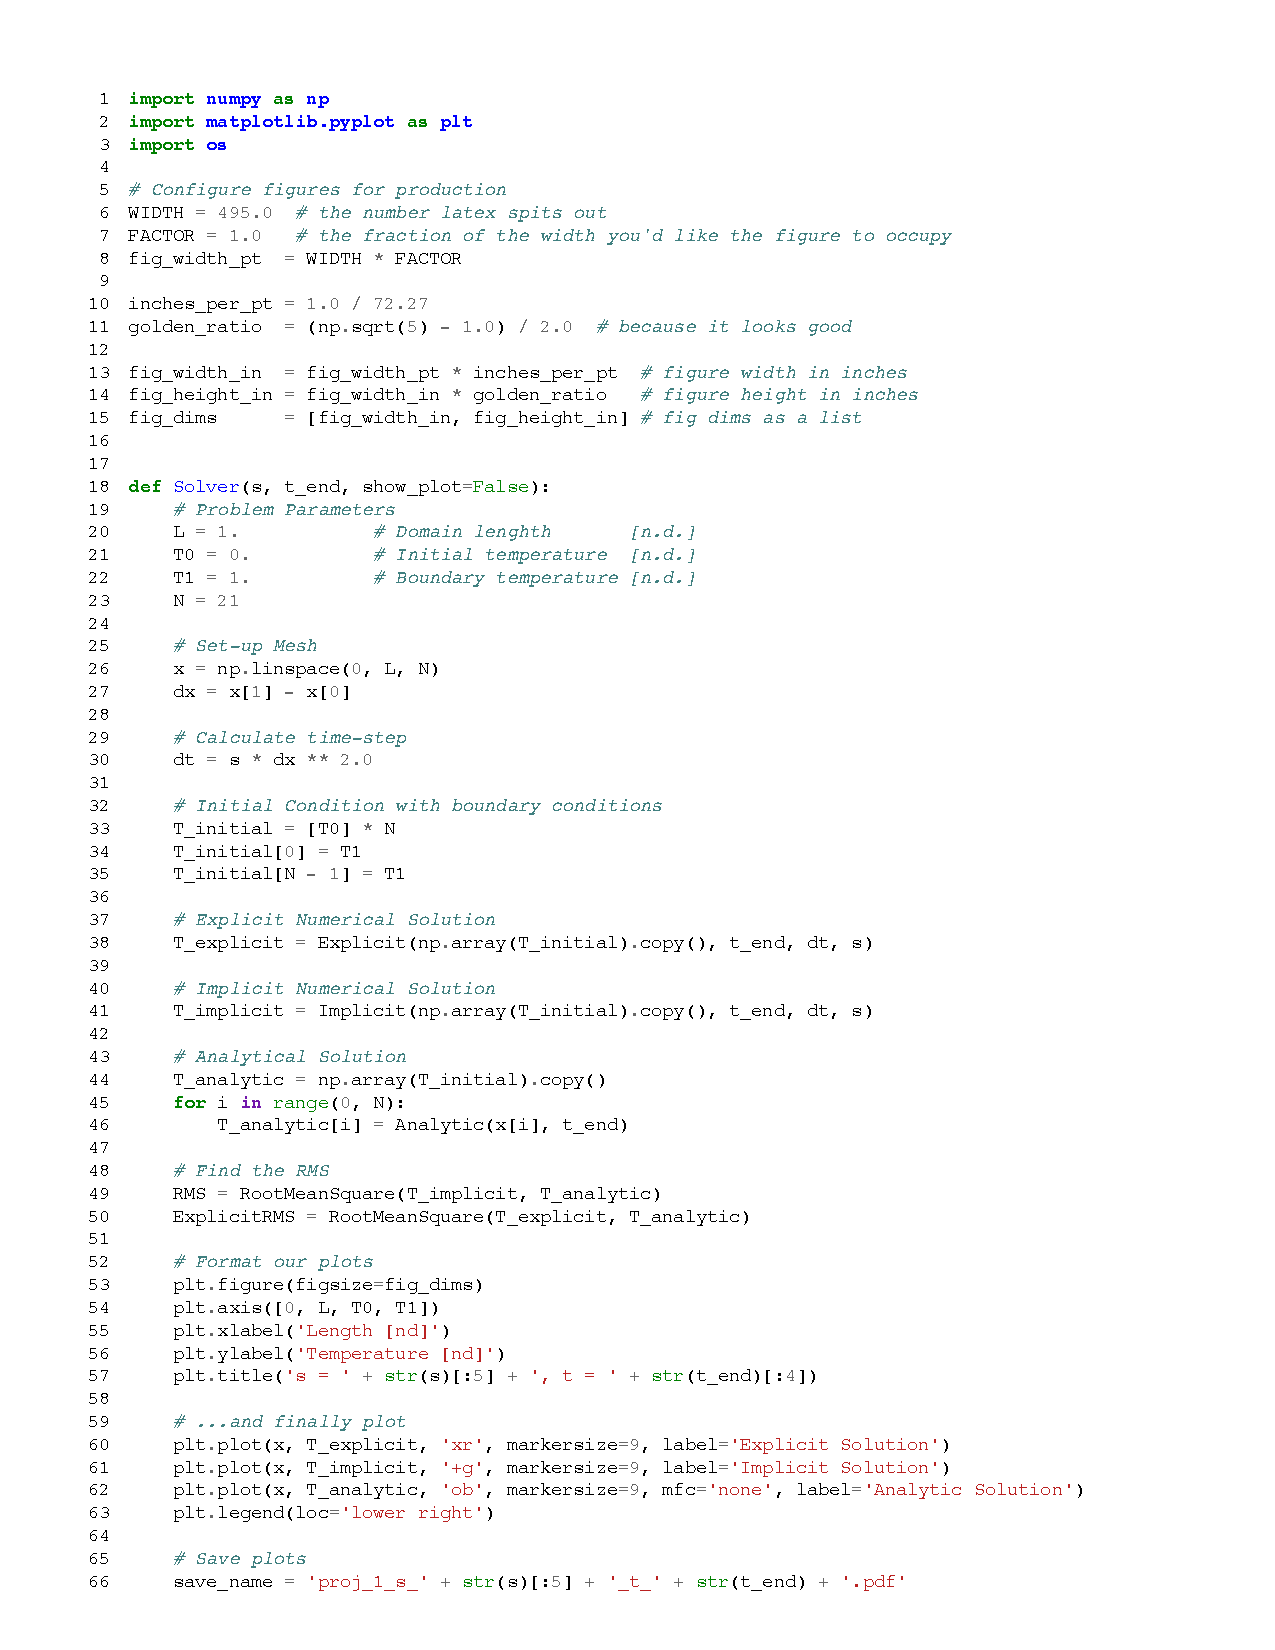
\includegraphics[page=1,width=0.93\textwidth]{../Karasinski - Case Study 1.pdf}
\end{center}
\end{figure}

\begin{figure}[htb]
\begin{center}
\includegraphics[page=2,width=0.93\textwidth]{../Karasinski - Case Study 1.pdf}
\end{center}
\end{figure}

\begin{figure}[htb]
\begin{center}
\includegraphics[page=3,width=0.93\textwidth]{../Karasinski - Case Study 1.pdf}
\end{center}
\end{figure}

\begin{figure}[htb]
\begin{center}
\includegraphics[page=4,width=0.93\textwidth]{../Karasinski - Case Study 1.pdf}
\end{center}
\end{figure}
%%%%%%%%%%%%%%%%%%%%%%%%%%%%%%%%%%%%%%%%%%%%%%%%%%%%%%%%%%%%%%%%%%%%%%
%\section*{Appendix B: Head of Second Appendix}
%\subsection*{Subsection head in appendix}
%The equation counter is not reset in an appendix and the numbers will
%follow one continual sequence from the beginning of the article to the very end as shown in the following example.
%\begin{equation}
%a = b + c.
%\end{equation}

\end{document}
